\documentclass{standalone}
\usepackage{tikz}
\usetikzlibrary{patterns, positioning}


\begin{document}
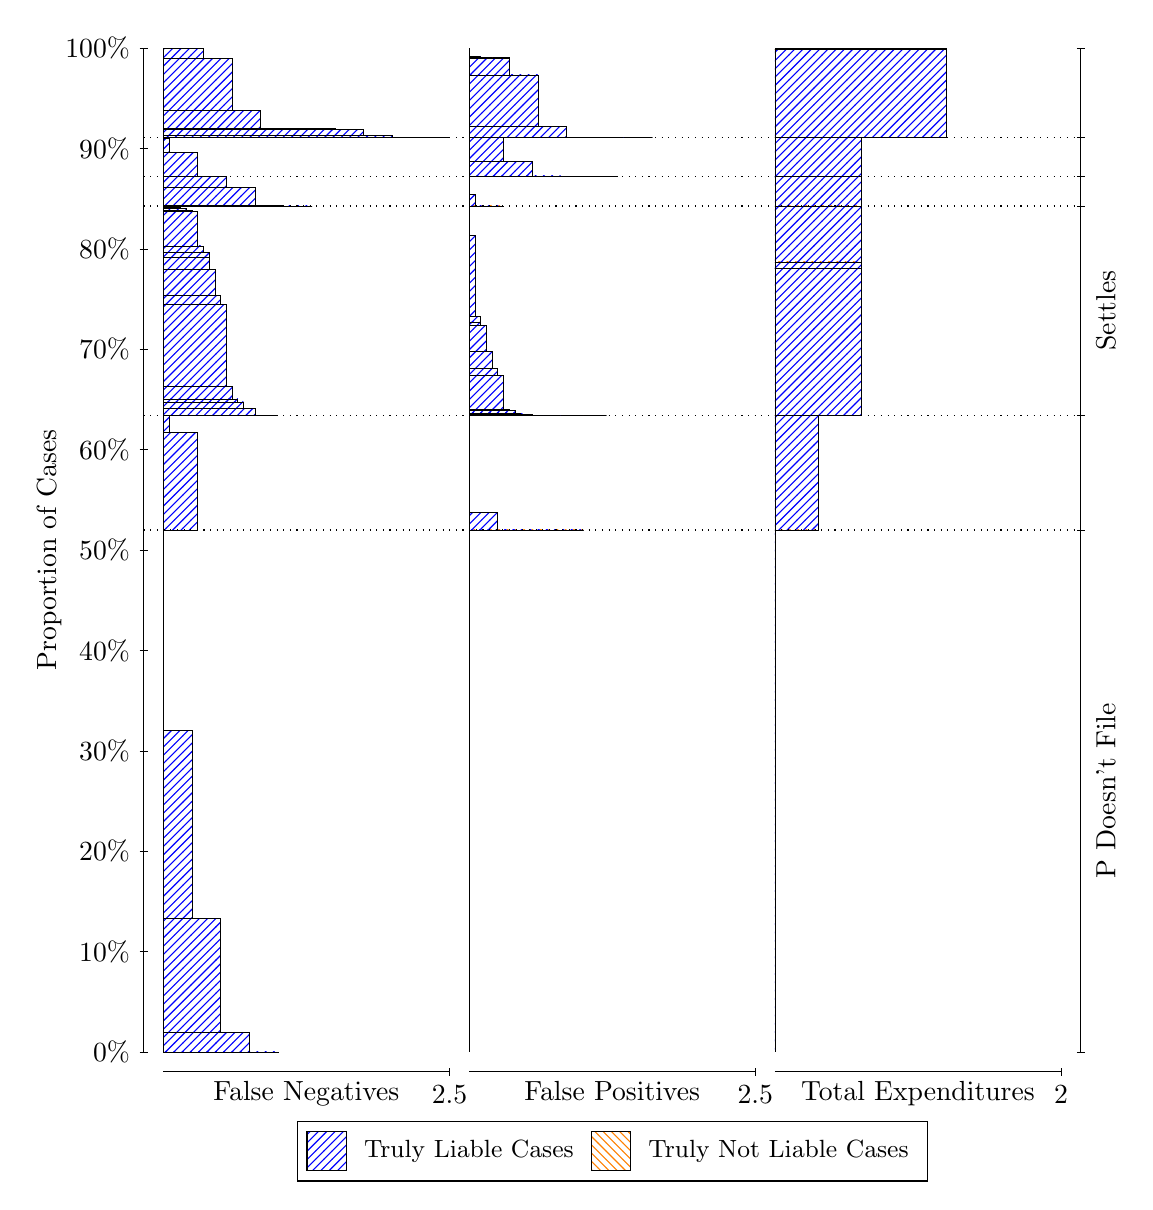
\begin{tikzpicture}
\draw[black, very thin] (1.5,1.75) -- (1.5,14.5);
\node[rotate=90, text=black, anchor=center] at (0.3, 8.125) {Proportion of Cases};
\draw[black, very thin] (1.45,1.75) -- (1.55,1.75);
\node[text=black, anchor=east] at (1.45, 1.75) {0\%};
\draw[black, very thin] (1.45,3.025) -- (1.55,3.025);
\node[text=black, anchor=east] at (1.45, 3.025) {10\%};
\draw[black, very thin] (1.45,4.3) -- (1.55,4.3);
\node[text=black, anchor=east] at (1.45, 4.3) {20\%};
\draw[black, very thin] (1.45,5.575) -- (1.55,5.575);
\node[text=black, anchor=east] at (1.45, 5.575) {30\%};
\draw[black, very thin] (1.45,6.85) -- (1.55,6.85);
\node[text=black, anchor=east] at (1.45, 6.85) {40\%};
\draw[black, very thin] (1.45,8.125) -- (1.55,8.125);
\node[text=black, anchor=east] at (1.45, 8.125) {50\%};
\draw[black, very thin] (1.45,9.4) -- (1.55,9.4);
\node[text=black, anchor=east] at (1.45, 9.4) {60\%};
\draw[black, very thin] (1.45,10.675) -- (1.55,10.675);
\node[text=black, anchor=east] at (1.45, 10.675) {70\%};
\draw[black, very thin] (1.45,11.95) -- (1.55,11.95);
\node[text=black, anchor=east] at (1.45, 11.95) {80\%};
\draw[black, very thin] (1.45,13.225) -- (1.55,13.225);
\node[text=black, anchor=east] at (1.45, 13.225) {90\%};
\draw[black, very thin] (1.45,14.5) -- (1.55,14.5);
\node[text=black, anchor=east] at (1.45, 14.5) {100\%};

\draw[black, very thin] (13.4,1.75) -- (13.4,14.5);
\draw[black, very thin] (13.35,1.75) -- (13.45,1.75);
\node[anchor=west] at (13.35, 1.75) {};
\draw[black, very thin] (13.35,8.3795) -- (13.45,8.3795);
\node[anchor=west] at (13.35, 8.3795) {};
\draw[black, very thin] (13.35,9.8386) -- (13.45,9.8386);
\node[anchor=west] at (13.35, 9.8386) {};
\draw[black, very thin] (13.35,12.494) -- (13.45,12.494);
\node[anchor=west] at (13.35, 12.494) {};
\draw[black, very thin] (13.35,12.868) -- (13.45,12.868);
\node[anchor=west] at (13.35, 12.868) {};
\draw[black, very thin] (13.35,13.366) -- (13.45,13.366);
\node[anchor=west] at (13.35, 13.366) {};
\draw[black, very thin] (13.35,14.5) -- (13.45,14.5);
\node[anchor=west] at (13.35, 14.5) {};

\draw[black, very thin, pattern color=blue, pattern=north east lines] (1.75,1.75) rectangle (3.2033,1.7525);
\draw[black, very thin, pattern color=blue, pattern=north east lines] (1.75,1.7525) rectangle (2.84,1.9968);
\draw[black, very thin, pattern color=blue, pattern=north east lines] (1.75,1.9968) rectangle (2.4767,3.4454);
\draw[black, very thin, pattern color=blue, pattern=north east lines] (1.75,3.4454) rectangle (2.1133,5.8311);
\draw[black, very thin, pattern color=orange, pattern=north west lines] (1.75,5.8311) rectangle (1.75,5.8311);
\draw[black, very thin, pattern color=blue, pattern=north east lines] (1.75,5.8311) rectangle (1.75,8.3795);
\draw[black, very thin, pattern color=blue, pattern=north east lines] (1.75,8.3795) rectangle (2.186,9.6197);
\draw[black, very thin, pattern color=blue, pattern=north east lines] (1.75,9.6197) rectangle (1.8227,9.8377);
\draw[black, very thin, pattern color=orange, pattern=north west lines] (1.75,9.8377) rectangle (1.75,9.8377);
\draw[black, very thin, pattern color=blue, pattern=north east lines] (1.75,9.8377) rectangle (1.75,9.8386);
\draw[black, very thin, pattern color=blue, pattern=north east lines] (1.75,9.8386) rectangle (3.2033,9.8386);
\draw[black, very thin, pattern color=blue, pattern=north east lines] (1.75,9.8386) rectangle (3.058,9.8387);
\draw[black, very thin, pattern color=blue, pattern=north east lines] (1.75,9.8387) rectangle (2.9127,9.9222);
\draw[black, very thin, pattern color=blue, pattern=north east lines] (1.75,9.9222) rectangle (2.84,9.9277);
\draw[black, very thin, pattern color=blue, pattern=north east lines] (1.75,9.9277) rectangle (2.7673,10.006);
\draw[black, very thin, pattern color=blue, pattern=north east lines] (1.75,10.006) rectangle (2.6947,10.044);
\draw[black, very thin, pattern color=blue, pattern=north east lines] (1.75,10.044) rectangle (2.622,10.21);
\draw[black, very thin, pattern color=blue, pattern=north east lines] (1.75,10.21) rectangle (2.5493,11.242);
\draw[black, very thin, pattern color=blue, pattern=north east lines] (1.75,11.242) rectangle (2.4767,11.354);
\draw[black, very thin, pattern color=blue, pattern=north east lines] (1.75,11.354) rectangle (2.404,11.688);
\draw[black, very thin, pattern color=blue, pattern=north east lines] (1.75,11.688) rectangle (2.3313,11.84);
\draw[black, very thin, pattern color=blue, pattern=north east lines] (1.75,11.84) rectangle (2.3313,11.903);
\draw[black, very thin, pattern color=blue, pattern=north east lines] (1.75,11.903) rectangle (2.2587,11.988);
\draw[black, very thin, pattern color=blue, pattern=north east lines] (1.75,11.988) rectangle (2.186,12.426);
\draw[black, very thin, pattern color=blue, pattern=north east lines] (1.75,12.426) rectangle (2.1133,12.435);
\draw[black, very thin, pattern color=blue, pattern=north east lines] (1.75,12.435) rectangle (2.0407,12.466);
\draw[black, very thin, pattern color=blue, pattern=north east lines] (1.75,12.466) rectangle (1.968,12.473);
\draw[black, very thin, pattern color=blue, pattern=north east lines] (1.75,12.473) rectangle (1.968,12.48);
\draw[black, very thin, pattern color=blue, pattern=north east lines] (1.75,12.48) rectangle (1.8953,12.484);
\draw[black, very thin, pattern color=blue, pattern=north east lines] (1.75,12.484) rectangle (1.8227,12.494);
\draw[black, very thin, pattern color=orange, pattern=north west lines] (1.75,12.494) rectangle (1.75,12.494);
\draw[black, very thin, pattern color=blue, pattern=north east lines] (1.75,12.494) rectangle (1.75,12.494);
\draw[black, very thin, pattern color=blue, pattern=north east lines] (1.75,12.494) rectangle (3.6393,12.494);
\draw[black, very thin, pattern color=blue, pattern=north east lines] (1.75,12.494) rectangle (3.276,12.504);
\draw[black, very thin, pattern color=blue, pattern=north east lines] (1.75,12.504) rectangle (2.9127,12.726);
\draw[black, very thin, pattern color=blue, pattern=north east lines] (1.75,12.726) rectangle (2.5493,12.867);
\draw[black, very thin, pattern color=blue, pattern=north east lines] (1.75,12.867) rectangle (2.186,12.868);
\draw[black, very thin, pattern color=orange, pattern=north west lines] (1.75,12.868) rectangle (1.75,12.868);
\draw[black, very thin, pattern color=blue, pattern=north east lines] (1.75,12.868) rectangle (2.186,13.172);
\draw[black, very thin, pattern color=blue, pattern=north east lines] (1.75,13.172) rectangle (1.8227,13.36);
\draw[black, very thin, pattern color=orange, pattern=north west lines] (1.75,13.36) rectangle (1.75,13.36);
\draw[black, very thin, pattern color=blue, pattern=north east lines] (1.75,13.36) rectangle (1.75,13.366);
\draw[black, very thin, pattern color=blue, pattern=north east lines] (1.75,13.366) rectangle (5.3833,13.366);
\draw[black, very thin, pattern color=blue, pattern=north east lines] (1.75,13.366) rectangle (5.02,13.367);
\draw[black, very thin, pattern color=blue, pattern=north east lines] (1.75,13.367) rectangle (4.6567,13.392);
\draw[black, very thin, pattern color=blue, pattern=north east lines] (1.75,13.392) rectangle (4.2933,13.471);
\draw[black, very thin, pattern color=blue, pattern=north east lines] (1.75,13.471) rectangle (3.93,13.476);
\draw[black, very thin, pattern color=blue, pattern=north east lines] (1.75,13.476) rectangle (3.712,13.476);
\draw[black, very thin, pattern color=blue, pattern=north east lines] (1.75,13.476) rectangle (3.5667,13.476);
\draw[black, very thin, pattern color=blue, pattern=north east lines] (1.75,13.476) rectangle (3.3487,13.481);
\draw[black, very thin, pattern color=blue, pattern=north east lines] (1.75,13.481) rectangle (3.2033,13.481);
\draw[black, very thin, pattern color=blue, pattern=north east lines] (1.75,13.481) rectangle (2.9853,13.708);
\draw[black, very thin, pattern color=blue, pattern=north east lines] (1.75,13.708) rectangle (2.622,14.364);
\draw[black, very thin, pattern color=blue, pattern=north east lines] (1.75,14.364) rectangle (2.2587,14.496);
\draw[black, very thin, pattern color=blue, pattern=north east lines] (1.75,14.496) rectangle (1.8953,14.5);
\draw[black, very thin, pattern color=orange, pattern=north west lines] (1.75,14.5) rectangle (1.75,14.5);
\draw[black, very thin, pattern color=blue, pattern=north east lines] (1.75,14.5) rectangle (1.75,14.5);
\draw[black, very thin, pattern color=orange, pattern=north west lines] (5.6333,1.75) rectangle (5.6333,1.75);
\draw[black, very thin, pattern color=blue, pattern=north east lines] (5.6333,1.75) rectangle (5.6333,8.3795);
\draw[black, very thin, pattern color=orange, pattern=north west lines] (5.6333,8.3795) rectangle (7.0867,8.3795);
\draw[black, very thin, pattern color=blue, pattern=north east lines] (5.6333,8.3795) rectangle (7.0867,8.3795);
\draw[black, very thin, pattern color=blue, pattern=north east lines] (5.6333,8.3795) rectangle (6.7233,8.3795);
\draw[black, very thin, pattern color=blue, pattern=north east lines] (5.6333,8.3795) rectangle (6.36,8.3804);
\draw[black, very thin, pattern color=blue, pattern=north east lines] (5.6333,8.3804) rectangle (5.9967,8.5983);
\draw[black, very thin, pattern color=blue, pattern=north east lines] (5.6333,8.5983) rectangle (5.6333,9.8386);
\draw[black, very thin, pattern color=orange, pattern=north west lines] (5.6333,9.8386) rectangle (7.3773,9.8386);
\draw[black, very thin, pattern color=blue, pattern=north east lines] (5.6333,9.8386) rectangle (7.3773,9.8386);
\draw[black, very thin, pattern color=orange, pattern=north west lines] (5.6333,9.8386) rectangle (7.232,9.8386);
\draw[black, very thin, pattern color=blue, pattern=north east lines] (5.6333,9.8386) rectangle (7.232,9.8386);
\draw[black, very thin, pattern color=orange, pattern=north west lines] (5.6333,9.8386) rectangle (7.0867,9.8386);
\draw[black, very thin, pattern color=blue, pattern=north east lines] (5.6333,9.8386) rectangle (7.0867,9.8386);
\draw[black, very thin, pattern color=blue, pattern=north east lines] (5.6333,9.8386) rectangle (7.014,9.8386);
\draw[black, very thin, pattern color=orange, pattern=north west lines] (5.6333,9.8386) rectangle (6.9413,9.8386);
\draw[black, very thin, pattern color=blue, pattern=north east lines] (5.6333,9.8386) rectangle (6.9413,9.8386);
\draw[black, very thin, pattern color=blue, pattern=north east lines] (5.6333,9.8386) rectangle (6.8687,9.8386);
\draw[black, very thin, pattern color=orange, pattern=north west lines] (5.6333,9.8386) rectangle (6.796,9.8386);
\draw[black, very thin, pattern color=blue, pattern=north east lines] (5.6333,9.8386) rectangle (6.796,9.8386);
\draw[black, very thin, pattern color=blue, pattern=north east lines] (5.6333,9.8386) rectangle (6.7233,9.8386);
\draw[black, very thin, pattern color=orange, pattern=north west lines] (5.6333,9.8386) rectangle (6.6507,9.8386);
\draw[black, very thin, pattern color=blue, pattern=north east lines] (5.6333,9.8386) rectangle (6.6507,9.8386);
\draw[black, very thin, pattern color=blue, pattern=north east lines] (5.6333,9.8386) rectangle (6.578,9.8386);
\draw[black, very thin, pattern color=blue, pattern=north east lines] (5.6333,9.8386) rectangle (6.5053,9.8387);
\draw[black, very thin, pattern color=orange, pattern=north west lines] (5.6333,9.8387) rectangle (6.5053,9.8387);
\draw[black, very thin, pattern color=blue, pattern=north east lines] (5.6333,9.8387) rectangle (6.5053,9.8387);
\draw[black, very thin, pattern color=blue, pattern=north east lines] (5.6333,9.8387) rectangle (6.4327,9.8485);
\draw[black, very thin, pattern color=blue, pattern=north east lines] (5.6333,9.8485) rectangle (6.36,9.8523);
\draw[black, very thin, pattern color=blue, pattern=north east lines] (5.6333,9.8523) rectangle (6.2873,9.8662);
\draw[black, very thin, pattern color=blue, pattern=north east lines] (5.6333,9.8662) rectangle (6.2147,9.8975);
\draw[black, very thin, pattern color=blue, pattern=north east lines] (5.6333,9.8975) rectangle (6.142,9.9027);
\draw[black, very thin, pattern color=blue, pattern=north east lines] (5.6333,9.9027) rectangle (6.142,9.9064);
\draw[black, very thin, pattern color=blue, pattern=north east lines] (5.6333,9.9064) rectangle (6.0693,10.345);
\draw[black, very thin, pattern color=blue, pattern=north east lines] (5.6333,10.345) rectangle (5.9967,10.429);
\draw[black, very thin, pattern color=blue, pattern=north east lines] (5.6333,10.429) rectangle (5.924,10.645);
\draw[black, very thin, pattern color=blue, pattern=north east lines] (5.6333,10.645) rectangle (5.8513,10.978);
\draw[black, very thin, pattern color=blue, pattern=north east lines] (5.6333,10.978) rectangle (5.7787,11.021);
\draw[black, very thin, pattern color=blue, pattern=north east lines] (5.6333,11.021) rectangle (5.7787,11.091);
\draw[black, very thin, pattern color=blue, pattern=north east lines] (5.6333,11.091) rectangle (5.706,12.123);
\draw[black, very thin, pattern color=blue, pattern=north east lines] (5.6333,12.123) rectangle (5.6333,12.494);
\draw[black, very thin, pattern color=orange, pattern=north west lines] (5.6333,12.494) rectangle (6.0693,12.494);
\draw[black, very thin, pattern color=blue, pattern=north east lines] (5.6333,12.494) rectangle (6.0693,12.496);
\draw[black, very thin, pattern color=blue, pattern=north east lines] (5.6333,12.496) rectangle (5.706,12.637);
\draw[black, very thin, pattern color=blue, pattern=north east lines] (5.6333,12.637) rectangle (5.6333,12.868);
\draw[black, very thin, pattern color=orange, pattern=north west lines] (5.6333,12.868) rectangle (7.5227,12.868);
\draw[black, very thin, pattern color=blue, pattern=north east lines] (5.6333,12.868) rectangle (7.5227,12.868);
\draw[black, very thin, pattern color=blue, pattern=north east lines] (5.6333,12.868) rectangle (7.1593,12.868);
\draw[black, very thin, pattern color=blue, pattern=north east lines] (5.6333,12.868) rectangle (6.796,12.875);
\draw[black, very thin, pattern color=blue, pattern=north east lines] (5.6333,12.875) rectangle (6.4327,13.063);
\draw[black, very thin, pattern color=blue, pattern=north east lines] (5.6333,13.063) rectangle (6.0693,13.366);
\draw[black, very thin, pattern color=orange, pattern=north west lines] (5.6333,13.366) rectangle (7.9587,13.366);
\draw[black, very thin, pattern color=blue, pattern=north east lines] (5.6333,13.366) rectangle (7.9587,13.366);
\draw[black, very thin, pattern color=orange, pattern=north west lines] (5.6333,13.366) rectangle (7.5953,13.366);
\draw[black, very thin, pattern color=blue, pattern=north east lines] (5.6333,13.366) rectangle (7.5953,13.366);
\draw[black, very thin, pattern color=orange, pattern=north west lines] (5.6333,13.366) rectangle (7.232,13.366);
\draw[black, very thin, pattern color=blue, pattern=north east lines] (5.6333,13.366) rectangle (7.232,13.37);
\draw[black, very thin, pattern color=blue, pattern=north east lines] (5.6333,13.37) rectangle (6.8687,13.502);
\draw[black, very thin, pattern color=orange, pattern=north west lines] (5.6333,13.502) rectangle (6.8687,13.502);
\draw[black, very thin, pattern color=blue, pattern=north east lines] (5.6333,13.502) rectangle (6.8687,13.502);
\draw[black, very thin, pattern color=blue, pattern=north east lines] (5.6333,13.502) rectangle (6.5053,14.157);
\draw[black, very thin, pattern color=blue, pattern=north east lines] (5.6333,14.157) rectangle (6.5053,14.158);
\draw[black, very thin, pattern color=blue, pattern=north east lines] (5.6333,14.158) rectangle (6.142,14.369);
\draw[black, very thin, pattern color=blue, pattern=north east lines] (5.6333,14.369) rectangle (6.142,14.385);
\draw[black, very thin, pattern color=orange, pattern=north west lines] (5.6333,14.385) rectangle (5.924,14.385);
\draw[black, very thin, pattern color=blue, pattern=north east lines] (5.6333,14.385) rectangle (5.924,14.385);
\draw[black, very thin, pattern color=blue, pattern=north east lines] (5.6333,14.385) rectangle (5.7787,14.39);
\draw[black, very thin, pattern color=blue, pattern=north east lines] (5.6333,14.39) rectangle (5.7787,14.39);
\draw[black, very thin, pattern color=orange, pattern=north west lines] (5.6333,14.39) rectangle (5.6333,14.39);
\draw[black, very thin, pattern color=blue, pattern=north east lines] (5.6333,14.39) rectangle (5.6333,14.5);
\draw[black, very thin, pattern color=orange, pattern=north west lines] (9.5167,1.75) rectangle (9.5167,1.75);
\draw[black, very thin, pattern color=blue, pattern=north east lines] (9.5167,1.75) rectangle (9.5167,8.3795);
\draw[black, very thin, pattern color=orange, pattern=north west lines] (9.5167,8.3795) rectangle (10.062,8.3795);
\draw[black, very thin, pattern color=blue, pattern=north east lines] (9.5167,8.3795) rectangle (10.062,9.8386);
\draw[black, very thin, pattern color=orange, pattern=north west lines] (9.5167,9.8386) rectangle (10.607,9.8386);
\draw[black, very thin, pattern color=blue, pattern=north east lines] (9.5167,9.8386) rectangle (10.607,11.704);
\draw[black, very thin, pattern color=orange, pattern=north west lines] (9.5167,11.704) rectangle (10.607,11.704);
\draw[black, very thin, pattern color=blue, pattern=north east lines] (9.5167,11.704) rectangle (10.607,11.783);
\draw[black, very thin, pattern color=orange, pattern=north west lines] (9.5167,11.783) rectangle (10.607,11.783);
\draw[black, very thin, pattern color=blue, pattern=north east lines] (9.5167,11.783) rectangle (10.607,12.494);
\draw[black, very thin, pattern color=orange, pattern=north west lines] (9.5167,12.494) rectangle (10.607,12.494);
\draw[black, very thin, pattern color=blue, pattern=north east lines] (9.5167,12.494) rectangle (10.607,12.868);
\draw[black, very thin, pattern color=orange, pattern=north west lines] (9.5167,12.868) rectangle (10.607,12.868);
\draw[black, very thin, pattern color=blue, pattern=north east lines] (9.5167,12.868) rectangle (10.607,13.366);
\draw[black, very thin, pattern color=orange, pattern=north west lines] (9.5167,13.366) rectangle (11.697,13.366);
\draw[black, very thin, pattern color=blue, pattern=north east lines] (9.5167,13.366) rectangle (11.697,14.482);
\draw[black, very thin, pattern color=orange, pattern=north west lines] (9.5167,14.482) rectangle (11.697,14.482);
\draw[black, very thin, pattern color=blue, pattern=north east lines] (9.5167,14.482) rectangle (11.697,14.5);
\draw[black, dotted] (1.5,8.3795) -- (13.4,8.3795);
\draw[black, dotted] (1.5,9.8386) -- (13.4,9.8386);
\draw[black, dotted] (1.5,12.494) -- (13.4,12.494);
\draw[black, dotted] (1.5,12.868) -- (13.4,12.868);
\draw[black, dotted] (1.5,13.366) -- (13.4,13.366);
\draw[black, very thin] (1.75,1.5) -- (5.3833,1.5);
\node[text=black, anchor=north] at (3.5667, 1.5) {False Negatives};
\draw[black, very thin] (5.3833,1.45) -- (5.3833,1.55);
\node[text=black, anchor=north] at (5.3833, 1.45) {2.5};

\draw[black, very thin] (5.6333,1.5) -- (9.2667,1.5);
\node[text=black, anchor=north] at (7.45, 1.5) {False Positives};
\draw[black, very thin] (9.2667,1.45) -- (9.2667,1.55);
\node[text=black, anchor=north] at (9.2667, 1.45) {2.5};

\draw[black, very thin] (9.5167,1.5) -- (13.15,1.5);
\node[text=black, anchor=north] at (11.333, 1.5) {Total Expenditures};
\draw[black, very thin] (13.15,1.45) -- (13.15,1.55);
\node[text=black, anchor=north] at (13.15, 1.45) {2};

\node[text=black, centered, rotate=90] at (13.72, 5.0647) {P Doesn't File};

\node[text=black, centered, rotate=90] at (13.72, 11.166) {Settles};




\draw (7.449999999999999,1.5) node[draw=none] (baseCoordinate) {};
\begin{scope}[align=center]
        \matrix[scale=0.5, draw=black, below=0.5cm of baseCoordinate, nodes={draw}, column sep=0.1cm]{
            \node[rectangle, draw, minimum width=0.5cm, minimum height=0.5cm, pattern color=blue, pattern=north east lines] {}; &
            \node[draw=none, font=\small, text=black] (B) {Truly Liable Cases}; &
            \node[rectangle, draw, minimum width=0.5cm, minimum height=0.5cm, pattern color=orange, pattern=north west lines] {}; &
            \node[draw=none, font=\small, text=black] (B) {Truly Not Liable Cases}; \\
            };
\end{scope}

\end{tikzpicture}
\end{document}